\chapter{Conclusion and Recommendations}
\label{ch:Conclusion}
The increasing population density in metropolitan areas,
coupled with the faster pace of everyday life, calls for the development of Inter-Urban Air Mobility (UAM) solutions.
Currently,
there is a gap in the market
since there is no competitor that can facilitate all market segments
and also provide \enquote*{last-mile transport} by air.
This is where the mission of this project comes into play, with the following objective:

“\textit{Design a low ground footprint, sustainable, urban transwing electric Vertical Take-Off and Landing vehicle within production costs of \qty{2}{M \texteuro}, by ten students in ten weeks time.}”

The final design achieved this objective, and its performance makes it a very competitive eVTOL.
The final design can be found in \Cref{fig_con:design_inhover} and \Cref{fig_con:Final_design_swing},
and its parameters can be found in \Cref{tab:conc_param}.
The biggest advantage of the \textit{Swing eVTOL} is its ground footprint of \qty{32}{m^2},
which is more than half the main competitors.
Furthermore,
its range is 1.4 times longer than the \textit{Joby S4} and more than three times as much as the \textit{Archer Midnight}.
Finally, it is also 10\% more energy efficient than \textit{Joby S4}, currently the most efficient eVTOL.
And all of these advantages come at a very competitive price,
making the \textit{Swing eVTOL} a very attractive aircraft for aircraft operators.

% This table is copied from the executive overview
\begin{table}[H]
\centering
\caption{Final design parameters of the \textit{Swing eVTOL.}}
\label{tab:conc_param}
    \sisetup{table-format=4, parse-numbers=false, input-decimal-markers=x}
    \begin{tabular}{
        l
        S
        >{\collectcell\unit}l<{\endcollectcell}
        |l
        S
        >{\collectcell\unit}l<{\endcollectcell}
    }
    \toprule
    MTOW          & 1643 & kg   & Wing span       &   14.0  & m   \\
    OEM           & 1243 & kg   & Wing area       &   14.0  & m^2 \\
    Range         &  250 & km   & MAC             &    1.06 & m   \\
    Payload       &  400 & kg   & Fuselage length &    8.0  & m   \\
    Battery mass  &  400 & kg   & No. Engines     &    6    & -   \\
    Cruise speed  &  200 & km/h & Battery energy  &    120  & kWh \\
    Stall speed   &  105 & km/h & No. Passengers  &    4    & -   \\
    Total Power   &  344 & kW   & Production Cost &    1.42    & M€  \\
    Consumed Power in Cruise   &  0.162 & kWh/km   & Ground Footprint &    32    & m^2  \\
    \bottomrule
    \end{tabular}
\end{table}
\begin{figure}[h]
  \centering  
\begin{subfigure}[b]{0.49\textwidth}
    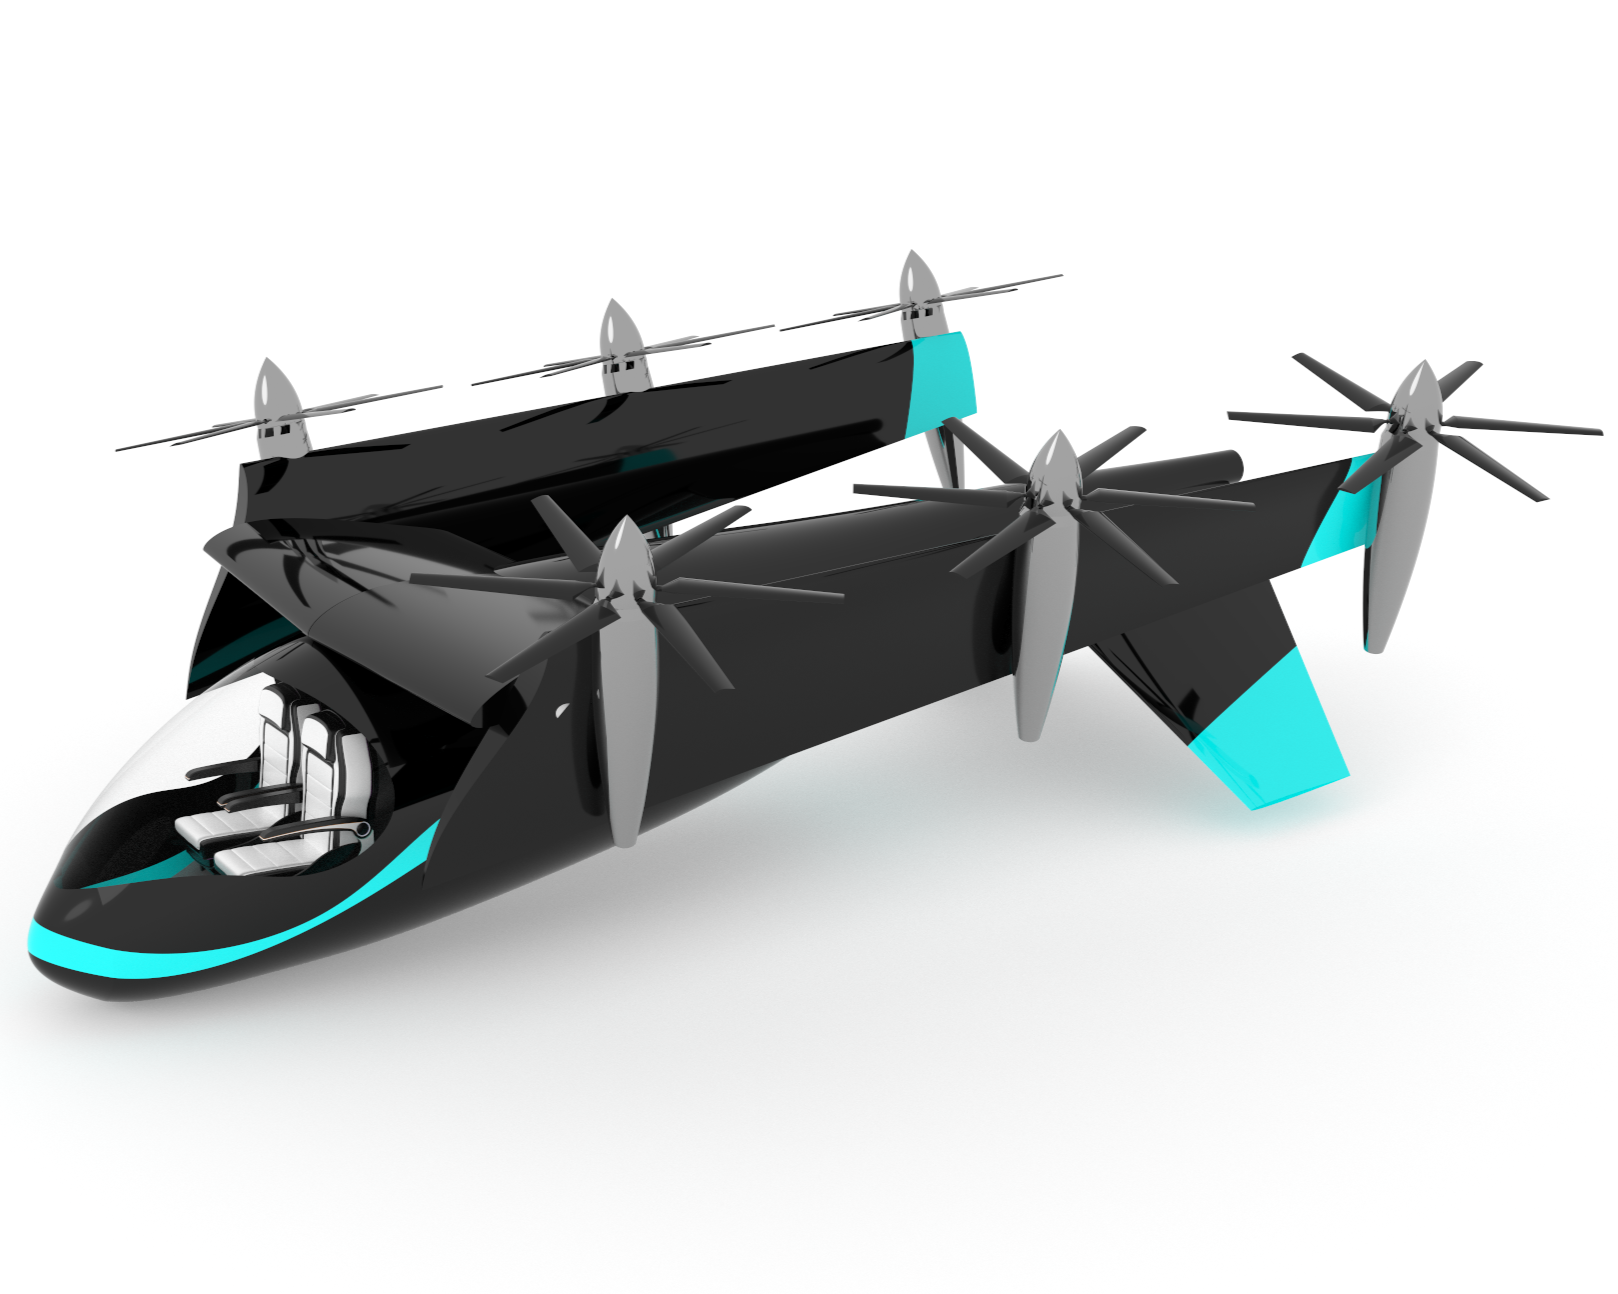
\includegraphics[width=1\linewidth]{Swing_eVTOL_ISO_hover.png}
    \caption{Final design of \textit{Swing eVTOL} in hover configuration}
    \label{fig_con:design_inhover}
\end{subfigure}
\begin{subfigure}[b]{0.49\textwidth}
    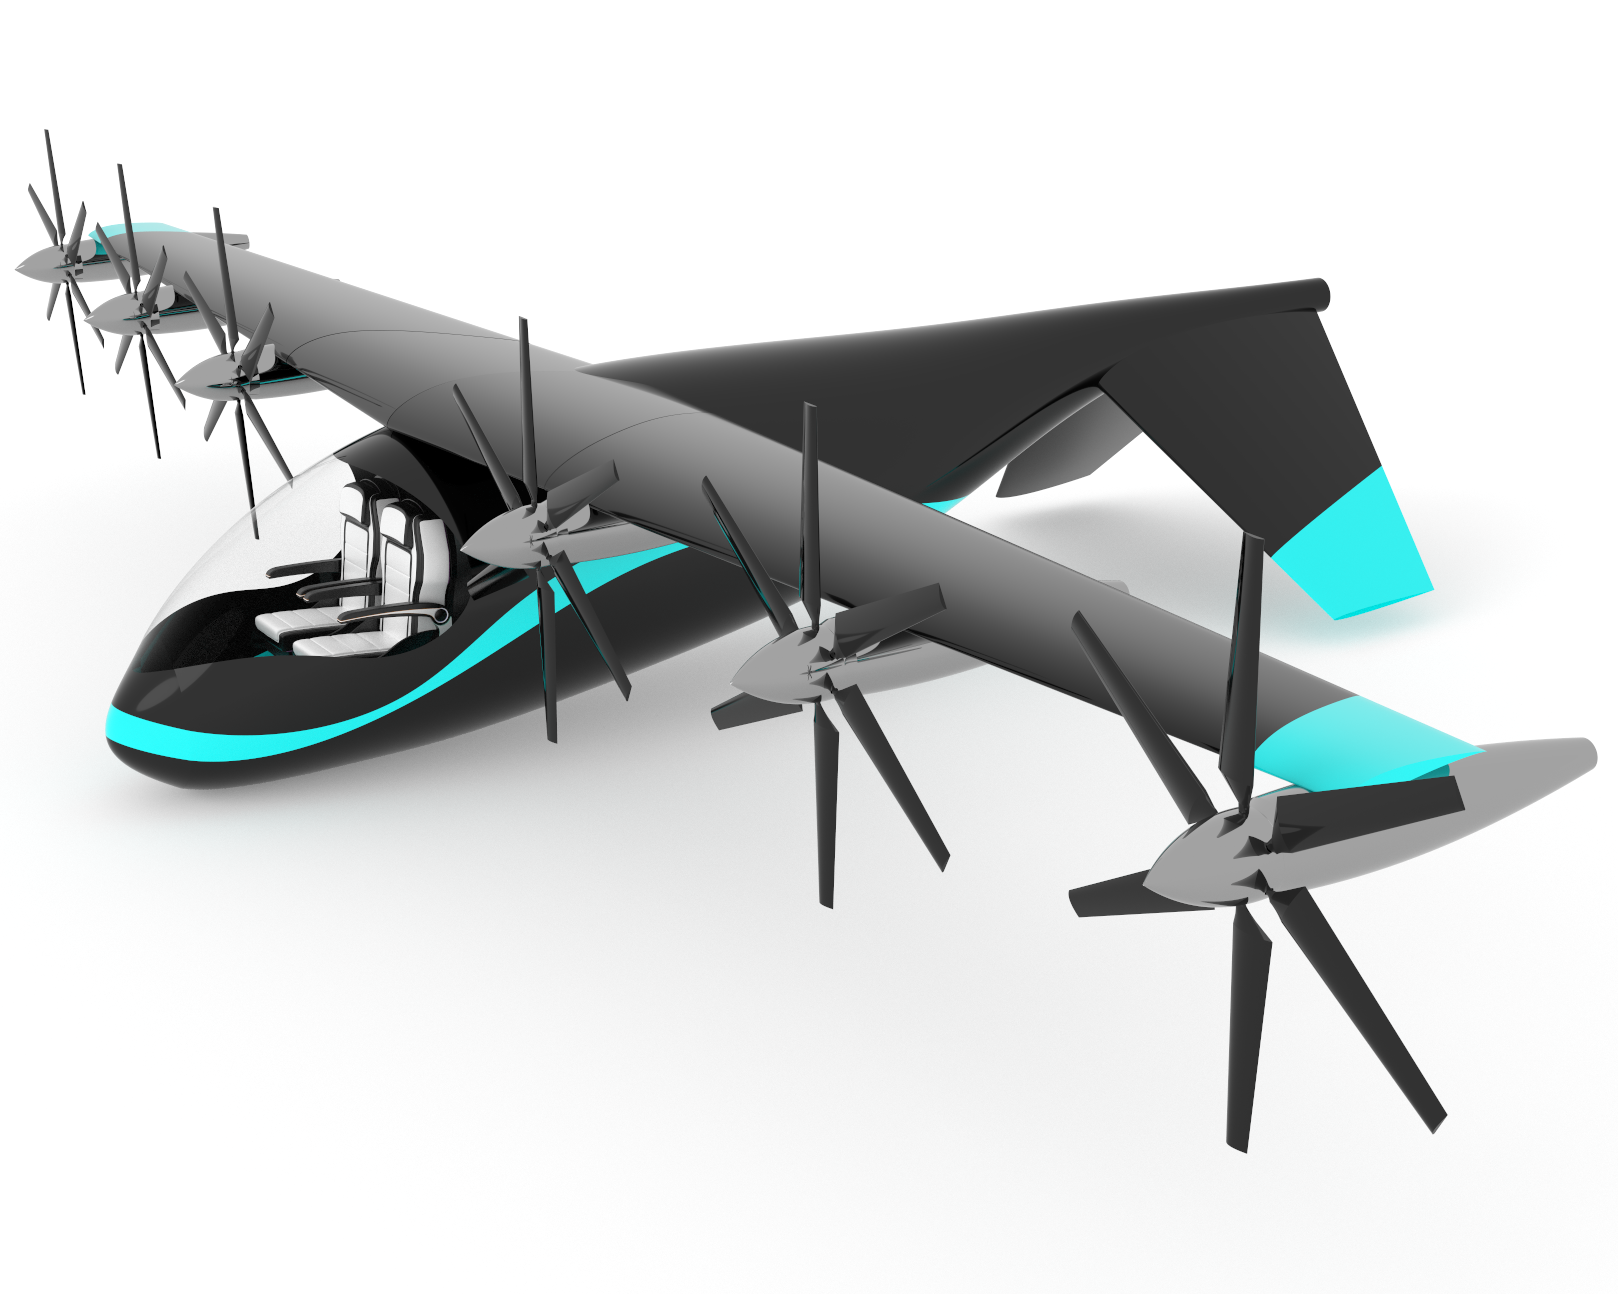
\includegraphics[width=1\linewidth]{Swing_eVTOL_ISO_cruise.png}
    \caption{Final design of \textit{Swing eVTOL} in cruise configuration}
    \label{fig_con:design_incruise}
\end{subfigure}
\caption{Final design of \textit{Swing eVTOL}}
\label{fig_con:Final_design_swing}
\end{figure}

Given the limited time available to produce this report, for each subsystem,
there are some recommendations to further develop the design of the \textit{Swing eVTOL}.
Firstly, for control and stability,
it is recommended
that another design iteration be done on the empennage and aircraft to improve the roll rate performance of the aircraft
as well as improving the spiral performance,
which is currently too unstable to be considered controllable.
Then, for the structure subsystem, it is recommended that the hinge is comprehensively sized also for dynamic loading,
since the report now only considers static loading.
For the electrical system, the next step is to look at the heat generated by the batteries
and to design a cooling system to deal with this heat properly.
The autonomous control can be improved by dynamic modelling for the different flight phases and tuning of the controllers.
Finally, it is recommended that for propulsion,
a Blade Element Momentum model is implemented since the current propeller sizing is based on empirical methods.

These recommendations aim to refine and optimise the already strong design,
ensuring that the \textit{Swing eVTOL} remains at the forefront of the emerging UAM market.